\subsection{Huffman}

Consider compressing the one byte data using the Huffman
(shortened to \textit{huff}) coding algorithm. This requires determining the
data's distribution on an initial pass. Then, the Huffman table is
recorded and each byte is encoded with its Huffman code. The problem is that
there is an overhead with storing the table.  Naively, one can store the table
by writing the number of entries in the table (1 byte) then each entry's symbol
(1 byte), code length (1 byte) and code (code length in bytes). See Figure
\ref{fig:huff-tab} for a picture. The resulting
table consumes
\begin{figure}
\centering\begin{tikzpicture}[node distance=0cm,start chain=1 going right] \footnotesize
  \tikzstyle{mytape}=[draw,minimum height=1.7cm]
	\node(A1)  [on chain=1,mytape,fill=blue!20] {$\underset{\text{entries}}{\underbrace{\overbracket{\text{ }m\text{ }}^{\text{1 byte}}}_{\text{number of}}}$};
	\node(B1)  [on chain=1,mytape,fill=yellow!20] {$\underbrace{\overbracket{s_1}^{\text{1 byte}}}_{\text{symbol 1}}$};
	\node(B2)  [on chain=1,mytape,fill=yellow!20] {$\underset{\text{of code 1}}{\underbrace{\overbracket{b_1}^{\text{1 byte}}}_{\text{bit length}}}$};
	\node(B3)  [on chain=1,mytape,fill=yellow!20] {$\overbracket{\underbrace{c_1}_{\text{code }1}}^{\lceil b_1/8\rceil\text{ bytes}}$};
	\node(D)   [on chain=1,mytape,fill=gray!20] {$\dots$};
	\node(C1)  [on chain=1,mytape,fill=yellow!20] {$\underbrace{\overbracket{s_m}^{\text{1 byte}}}_{\text{symbol m}}$};
	\node(C2)  [on chain=1,mytape,fill=yellow!20] {$\underset{\text{of code }m}{\underbrace{\overbracket{b_m}^{\text{1 byte}}}_{\text{bit length}}}$};
	\node(C3)  [on chain=1,mytape,fill=yellow!20] {$\overbracket{\underbrace{c_m}_{\text{code }m}}^{\lceil b_m/8\rceil\text{ bytes}}$};
\end{tikzpicture}
	\caption{\label{fig:huff-tab} The naive encoding of the Huffman table
where $c_i$ is the Huffman code of symbol $s_i$ with bit length $b_i$; $i$
ranges from 1 to $m$ (the number of table entries).}
\end{figure}


\[ 1 + 2m + \sum_{i=1}^m\lceil b_i / 8 \rceil \]
bytes where $m\in\mathbb{Z}\cap[0,255]$ is the number of entries in the table
and $b_i$ is the length of the $i$-th entry's code in bits. The number of
entries is the number of unique one byte values in the data.
If we use huff on the one byte zig-zag deltas of the vbbe21-zd encoding (let's name this strategy
\textit{huff-vbbe21-zd}), the number of entries is
dependent on the read's length. Short reads may only contain 100 unique one byte
deltas whilst long reads may easily contain more than 250 entries. If we
estimate that this is roughly 200 and the average code length is 2 bytes then
the table consumes
\[ 1 + 2\times 200 + 200\times 2 = 801 \]
bytes. The maximum number of entries is 256 so the maximum table size is roughly
1025 bytes.

However, rather than encoding the exact Huffman table for each read and consuming
roughly 800 bytes in storage, it makes more
sense to use a shared Huffman table which approximates the zig-zag delta
distribution of most reads well. We are at an advantage here in that the zig-zag
deltas follow a similar distribution between reads.
%These are bytes we don't need to repeat in each read when each read has a similar distribution of zig-zag deltas.
For example, 0 is the most common zig-zag delta among reads so naturally its code will
have the fewest number of bits and this will be efficient for the majority of
reads. One simple approach is to construct the optimal Huffman table for the
whole data set of zig-zag deltas. Then, we can store the code table once in the
source code and encode each read using the same table. Let's call this method
the static Huffman algorithm which is being applied to the one byte zig-zag
deltas, so \textit{shuff-vbbe21-zd} for short. This table consumes
1042 bytes but we can store it statically alongside the source code, so unless
we are considering the Kolmogorov complexity of the data its size is not
calculated in the compression size. The distribution of code lengths from this
table is shown in Figure \ref{fig:shuff-len}. The figure shows the distribution
splits into two alternating distributions from about 116 onwards which
represents the higher frequency of large positive compared to large negative
deltas, as previously discussed.

huff-vbbe21-zd consumes more space than the shuff-vbbe21-zd algorithm since it
records a different Huffman table for each read in the compressed data. The
space consumed by the Huffman table turns out to be more than the size difference
between the globally approximated and read-optimal Huffman encoding of the
zig-zag deltas.
%TODO See the results section for the details.
%For example, on the data set
%huff applied to vbe21 (hereafter \textit{huff-vbe21}) consumes 36.10 GiB versus
%35.85 GiB for shuff-vbe21 which is a difference of $\sim537$ bytes per read.
%This results is a compression ratio of 2.927 versus 2.948.
%%Moreover, when applied to a different human DNA data set huff-vbe21 consumes
Furthermore, huff-vbbe21-zd takes longer than shuff-vbbe21-zd during compression and decompression.
During compression, huff-vbbe21-zd must do an initial pass of the read to count the data's
frequencies and then construct the Huffman tree and table. During
decompression, huff-vbbe21-zd must read the table and construct the tree before decoding
the data. shuff-vbbe21-zd doesn't need to perform any of these operations since it
pre-calculates the shared table and tree and stores them in static memory.

During compression, calculating the frequencies takes $O(n)$ time. Then,
constructing the tree takes $O(x^2\log x)$ time using the bottom-up construction
% TODO add reference here
algorithm where $0\le x \le 256$ is the number of unique bytes or exceptions
when being applied to vbe21. Constructing the table requires traversing each
branch on the tree which takes $O(x)$ time since there are $2x-1$ nodes in a
Huffman tree. Then, recording the table takes $O(x)$ time and encoding the bytes
takes $O(n)$ time using the table. In total, the huff-vbbe21-zd algorithm takes
$O(n + x^2\log x)$ time for compression while shuff-vbbe21-zd takes $O(n)$ time. Compared
to $n$, the size of the input, $x$ is usually a lot smaller so it has a small
but true effect on the compression time.

During decompression, huff-vbbe21-zd take $O(n + x)$ time since it must construct the tree
whilst shuff-vbbe21-zd takes $O(n)$ time. But in practicality they take the same time. All
in all, as long as there is a space benefit to using shuff-vbbe21-zd, which there usually
is if the approximation is good, there is no reason to using huff-vbbe21-zd since shuff-vbbe21-zd is
faster during compression and decompression.

\begin{figure}
	\centering
% Created by tikzDevice version 0.12.3.1 on 2022-10-12 14:52:31
% !TEX encoding = UTF-8 Unicode
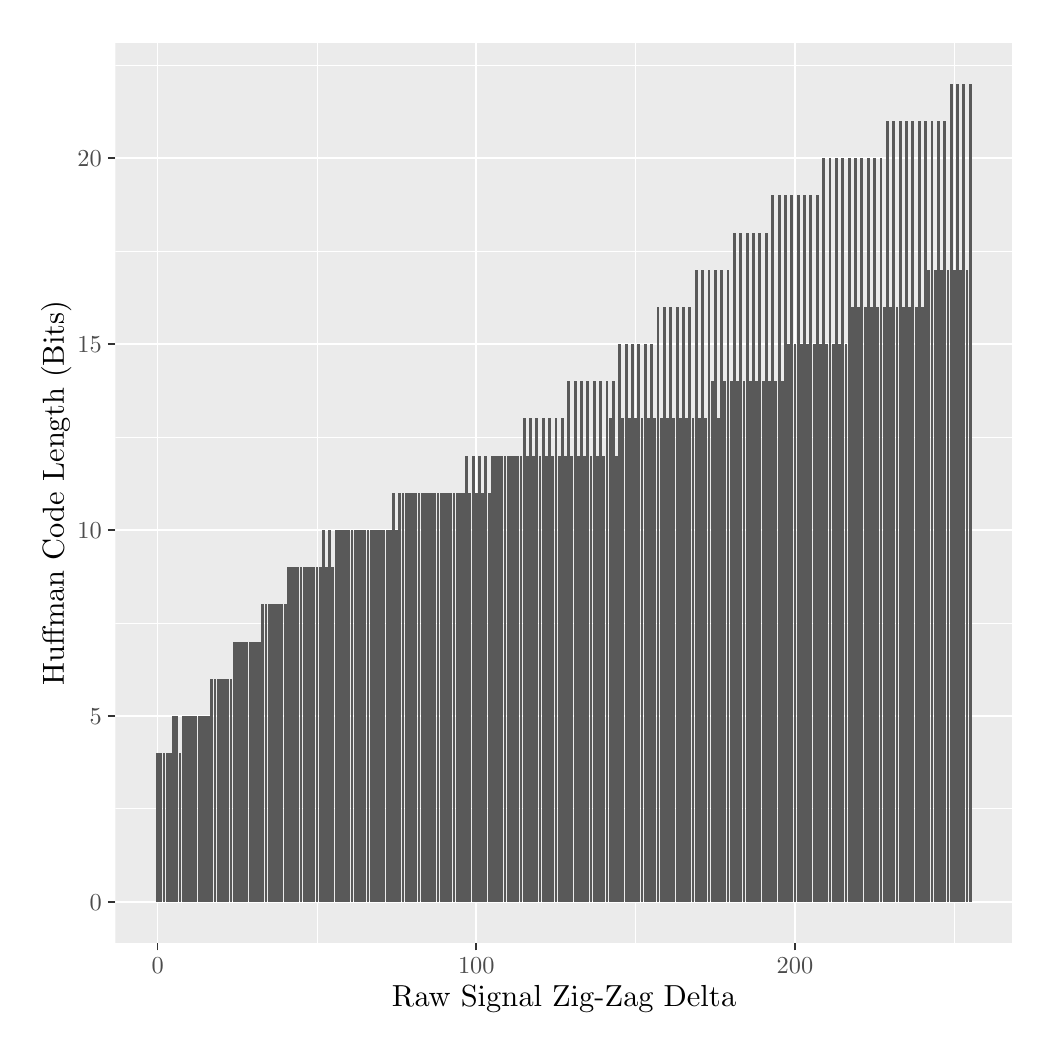
\begin{tikzpicture}[x=1pt,y=1pt]
\definecolor{fillColor}{RGB}{255,255,255}
\path[use as bounding box,fill=fillColor,fill opacity=0.00] (0,0) rectangle (361.35,361.35);
\begin{scope}
\path[clip] (  0.00,  0.00) rectangle (361.35,361.35);
\definecolor{drawColor}{RGB}{255,255,255}
\definecolor{fillColor}{RGB}{255,255,255}

\path[draw=drawColor,line width= 0.6pt,line join=round,line cap=round,fill=fillColor] (  0.00,  0.00) rectangle (361.35,361.35);
\end{scope}
\begin{scope}
\path[clip] ( 31.71, 30.69) rectangle (355.85,355.85);
\definecolor{fillColor}{gray}{0.92}

\path[fill=fillColor] ( 31.71, 30.69) rectangle (355.85,355.85);
\definecolor{drawColor}{RGB}{255,255,255}

\path[draw=drawColor,line width= 0.3pt,line join=round] ( 31.71, 79.06) --
	(355.85, 79.06);

\path[draw=drawColor,line width= 0.3pt,line join=round] ( 31.71,146.24) --
	(355.85,146.24);

\path[draw=drawColor,line width= 0.3pt,line join=round] ( 31.71,213.42) --
	(355.85,213.42);

\path[draw=drawColor,line width= 0.3pt,line join=round] ( 31.71,280.61) --
	(355.85,280.61);

\path[draw=drawColor,line width= 0.3pt,line join=round] ( 31.71,347.79) --
	(355.85,347.79);

\path[draw=drawColor,line width= 0.3pt,line join=round] (104.54, 30.69) --
	(104.54,355.85);

\path[draw=drawColor,line width= 0.3pt,line join=round] (219.69, 30.69) --
	(219.69,355.85);

\path[draw=drawColor,line width= 0.3pt,line join=round] (334.84, 30.69) --
	(334.84,355.85);

\path[draw=drawColor,line width= 0.6pt,line join=round] ( 31.71, 45.47) --
	(355.85, 45.47);

\path[draw=drawColor,line width= 0.6pt,line join=round] ( 31.71,112.65) --
	(355.85,112.65);

\path[draw=drawColor,line width= 0.6pt,line join=round] ( 31.71,179.83) --
	(355.85,179.83);

\path[draw=drawColor,line width= 0.6pt,line join=round] ( 31.71,247.01) --
	(355.85,247.01);

\path[draw=drawColor,line width= 0.6pt,line join=round] ( 31.71,314.20) --
	(355.85,314.20);

\path[draw=drawColor,line width= 0.6pt,line join=round] ( 46.96, 30.69) --
	( 46.96,355.85);

\path[draw=drawColor,line width= 0.6pt,line join=round] (162.11, 30.69) --
	(162.11,355.85);

\path[draw=drawColor,line width= 0.6pt,line join=round] (277.27, 30.69) --
	(277.27,355.85);
\definecolor{fillColor}{gray}{0.35}

\path[fill=fillColor] ( 46.45, 45.47) rectangle ( 47.48, 99.21);

\path[fill=fillColor] ( 47.60, 45.47) rectangle ( 48.63, 99.21);

\path[fill=fillColor] ( 48.75, 45.47) rectangle ( 49.79, 99.21);

\path[fill=fillColor] ( 49.90, 45.47) rectangle ( 50.94, 99.21);

\path[fill=fillColor] ( 51.05, 45.47) rectangle ( 52.09, 99.21);

\path[fill=fillColor] ( 52.20, 45.47) rectangle ( 53.24,112.65);

\path[fill=fillColor] ( 53.35, 45.47) rectangle ( 54.39,112.65);

\path[fill=fillColor] ( 54.51, 45.47) rectangle ( 55.54, 99.21);

\path[fill=fillColor] ( 55.66, 45.47) rectangle ( 56.69,112.65);

\path[fill=fillColor] ( 56.81, 45.47) rectangle ( 57.85,112.65);

\path[fill=fillColor] ( 57.96, 45.47) rectangle ( 59.00,112.65);

\path[fill=fillColor] ( 59.11, 45.47) rectangle ( 60.15,112.65);

\path[fill=fillColor] ( 60.26, 45.47) rectangle ( 61.30,112.65);

\path[fill=fillColor] ( 61.42, 45.47) rectangle ( 62.45,112.65);

\path[fill=fillColor] ( 62.57, 45.47) rectangle ( 63.60,112.65);

\path[fill=fillColor] ( 63.72, 45.47) rectangle ( 64.75,112.65);

\path[fill=fillColor] ( 64.87, 45.47) rectangle ( 65.91,112.65);

\path[fill=fillColor] ( 66.02, 45.47) rectangle ( 67.06,126.09);

\path[fill=fillColor] ( 67.17, 45.47) rectangle ( 68.21,126.09);

\path[fill=fillColor] ( 68.32, 45.47) rectangle ( 69.36,126.09);

\path[fill=fillColor] ( 69.48, 45.47) rectangle ( 70.51,126.09);

\path[fill=fillColor] ( 70.63, 45.47) rectangle ( 71.66,126.09);

\path[fill=fillColor] ( 71.78, 45.47) rectangle ( 72.82,126.09);

\path[fill=fillColor] ( 72.93, 45.47) rectangle ( 73.97,126.09);

\path[fill=fillColor] ( 74.08, 45.47) rectangle ( 75.12,139.52);

\path[fill=fillColor] ( 75.23, 45.47) rectangle ( 76.27,139.52);

\path[fill=fillColor] ( 76.38, 45.47) rectangle ( 77.42,139.52);

\path[fill=fillColor] ( 77.54, 45.47) rectangle ( 78.57,139.52);

\path[fill=fillColor] ( 78.69, 45.47) rectangle ( 79.72,139.52);

\path[fill=fillColor] ( 79.84, 45.47) rectangle ( 80.88,139.52);

\path[fill=fillColor] ( 80.99, 45.47) rectangle ( 82.03,139.52);

\path[fill=fillColor] ( 82.14, 45.47) rectangle ( 83.18,139.52);

\path[fill=fillColor] ( 83.29, 45.47) rectangle ( 84.33,139.52);

\path[fill=fillColor] ( 84.45, 45.47) rectangle ( 85.48,152.96);

\path[fill=fillColor] ( 85.60, 45.47) rectangle ( 86.63,152.96);

\path[fill=fillColor] ( 86.75, 45.47) rectangle ( 87.78,152.96);

\path[fill=fillColor] ( 87.90, 45.47) rectangle ( 88.94,152.96);

\path[fill=fillColor] ( 89.05, 45.47) rectangle ( 90.09,152.96);

\path[fill=fillColor] ( 90.20, 45.47) rectangle ( 91.24,152.96);

\path[fill=fillColor] ( 91.35, 45.47) rectangle ( 92.39,152.96);

\path[fill=fillColor] ( 92.51, 45.47) rectangle ( 93.54,152.96);

\path[fill=fillColor] ( 93.66, 45.47) rectangle ( 94.69,166.39);

\path[fill=fillColor] ( 94.81, 45.47) rectangle ( 95.85,166.39);

\path[fill=fillColor] ( 95.96, 45.47) rectangle ( 97.00,166.39);

\path[fill=fillColor] ( 97.11, 45.47) rectangle ( 98.15,166.39);

\path[fill=fillColor] ( 98.26, 45.47) rectangle ( 99.30,166.39);

\path[fill=fillColor] ( 99.42, 45.47) rectangle (100.45,166.39);

\path[fill=fillColor] (100.57, 45.47) rectangle (101.60,166.39);

\path[fill=fillColor] (101.72, 45.47) rectangle (102.75,166.39);

\path[fill=fillColor] (102.87, 45.47) rectangle (103.91,166.39);

\path[fill=fillColor] (104.02, 45.47) rectangle (105.06,166.39);

\path[fill=fillColor] (105.17, 45.47) rectangle (106.21,166.39);

\path[fill=fillColor] (106.32, 45.47) rectangle (107.36,179.83);

\path[fill=fillColor] (107.48, 45.47) rectangle (108.51,166.39);

\path[fill=fillColor] (108.63, 45.47) rectangle (109.66,179.83);

\path[fill=fillColor] (109.78, 45.47) rectangle (110.82,166.39);

\path[fill=fillColor] (110.93, 45.47) rectangle (111.97,179.83);

\path[fill=fillColor] (112.08, 45.47) rectangle (113.12,179.83);

\path[fill=fillColor] (113.23, 45.47) rectangle (114.27,179.83);

\path[fill=fillColor] (114.38, 45.47) rectangle (115.42,179.83);

\path[fill=fillColor] (115.54, 45.47) rectangle (116.57,179.83);

\path[fill=fillColor] (116.69, 45.47) rectangle (117.72,179.83);

\path[fill=fillColor] (117.84, 45.47) rectangle (118.88,179.83);

\path[fill=fillColor] (118.99, 45.47) rectangle (120.03,179.83);

\path[fill=fillColor] (120.14, 45.47) rectangle (121.18,179.83);

\path[fill=fillColor] (121.29, 45.47) rectangle (122.33,179.83);

\path[fill=fillColor] (122.45, 45.47) rectangle (123.48,179.83);

\path[fill=fillColor] (123.60, 45.47) rectangle (124.63,179.83);

\path[fill=fillColor] (124.75, 45.47) rectangle (125.78,179.83);

\path[fill=fillColor] (125.90, 45.47) rectangle (126.94,179.83);

\path[fill=fillColor] (127.05, 45.47) rectangle (128.09,179.83);

\path[fill=fillColor] (128.20, 45.47) rectangle (129.24,179.83);

\path[fill=fillColor] (129.35, 45.47) rectangle (130.39,179.83);

\path[fill=fillColor] (130.51, 45.47) rectangle (131.54,179.83);

\path[fill=fillColor] (131.66, 45.47) rectangle (132.69,193.27);

\path[fill=fillColor] (132.81, 45.47) rectangle (133.85,179.83);

\path[fill=fillColor] (133.96, 45.47) rectangle (135.00,193.27);

\path[fill=fillColor] (135.11, 45.47) rectangle (136.15,193.27);

\path[fill=fillColor] (136.26, 45.47) rectangle (137.30,193.27);

\path[fill=fillColor] (137.41, 45.47) rectangle (138.45,193.27);

\path[fill=fillColor] (138.57, 45.47) rectangle (139.60,193.27);

\path[fill=fillColor] (139.72, 45.47) rectangle (140.75,193.27);

\path[fill=fillColor] (140.87, 45.47) rectangle (141.91,193.27);

\path[fill=fillColor] (142.02, 45.47) rectangle (143.06,193.27);

\path[fill=fillColor] (143.17, 45.47) rectangle (144.21,193.27);

\path[fill=fillColor] (144.32, 45.47) rectangle (145.36,193.27);

\path[fill=fillColor] (145.48, 45.47) rectangle (146.51,193.27);

\path[fill=fillColor] (146.63, 45.47) rectangle (147.66,193.27);

\path[fill=fillColor] (147.78, 45.47) rectangle (148.81,193.27);

\path[fill=fillColor] (148.93, 45.47) rectangle (149.97,193.27);

\path[fill=fillColor] (150.08, 45.47) rectangle (151.12,193.27);

\path[fill=fillColor] (151.23, 45.47) rectangle (152.27,193.27);

\path[fill=fillColor] (152.38, 45.47) rectangle (153.42,193.27);

\path[fill=fillColor] (153.54, 45.47) rectangle (154.57,193.27);

\path[fill=fillColor] (154.69, 45.47) rectangle (155.72,193.27);

\path[fill=fillColor] (155.84, 45.47) rectangle (156.88,193.27);

\path[fill=fillColor] (156.99, 45.47) rectangle (158.03,193.27);

\path[fill=fillColor] (158.14, 45.47) rectangle (159.18,206.70);

\path[fill=fillColor] (159.29, 45.47) rectangle (160.33,193.27);

\path[fill=fillColor] (160.44, 45.47) rectangle (161.48,206.70);

\path[fill=fillColor] (161.60, 45.47) rectangle (162.63,193.27);

\path[fill=fillColor] (162.75, 45.47) rectangle (163.78,206.70);

\path[fill=fillColor] (163.90, 45.47) rectangle (164.94,193.27);

\path[fill=fillColor] (165.05, 45.47) rectangle (166.09,206.70);

\path[fill=fillColor] (166.20, 45.47) rectangle (167.24,193.27);

\path[fill=fillColor] (167.35, 45.47) rectangle (168.39,206.70);

\path[fill=fillColor] (168.51, 45.47) rectangle (169.54,206.70);

\path[fill=fillColor] (169.66, 45.47) rectangle (170.69,206.70);

\path[fill=fillColor] (170.81, 45.47) rectangle (171.84,206.70);

\path[fill=fillColor] (171.96, 45.47) rectangle (173.00,206.70);

\path[fill=fillColor] (173.11, 45.47) rectangle (174.15,206.70);

\path[fill=fillColor] (174.26, 45.47) rectangle (175.30,206.70);

\path[fill=fillColor] (175.41, 45.47) rectangle (176.45,206.70);

\path[fill=fillColor] (176.57, 45.47) rectangle (177.60,206.70);

\path[fill=fillColor] (177.72, 45.47) rectangle (178.75,206.70);

\path[fill=fillColor] (178.87, 45.47) rectangle (179.91,220.14);

\path[fill=fillColor] (180.02, 45.47) rectangle (181.06,206.70);

\path[fill=fillColor] (181.17, 45.47) rectangle (182.21,220.14);

\path[fill=fillColor] (182.32, 45.47) rectangle (183.36,206.70);

\path[fill=fillColor] (183.48, 45.47) rectangle (184.51,220.14);

\path[fill=fillColor] (184.63, 45.47) rectangle (185.66,206.70);

\path[fill=fillColor] (185.78, 45.47) rectangle (186.81,220.14);

\path[fill=fillColor] (186.93, 45.47) rectangle (187.97,206.70);

\path[fill=fillColor] (188.08, 45.47) rectangle (189.12,220.14);

\path[fill=fillColor] (189.23, 45.47) rectangle (190.27,206.70);

\path[fill=fillColor] (190.38, 45.47) rectangle (191.42,220.14);

\path[fill=fillColor] (191.54, 45.47) rectangle (192.57,206.70);

\path[fill=fillColor] (192.69, 45.47) rectangle (193.72,220.14);

\path[fill=fillColor] (193.84, 45.47) rectangle (194.88,206.70);

\path[fill=fillColor] (194.99, 45.47) rectangle (196.03,233.58);

\path[fill=fillColor] (196.14, 45.47) rectangle (197.18,206.70);

\path[fill=fillColor] (197.29, 45.47) rectangle (198.33,233.58);

\path[fill=fillColor] (198.44, 45.47) rectangle (199.48,206.70);

\path[fill=fillColor] (199.60, 45.47) rectangle (200.63,233.58);

\path[fill=fillColor] (200.75, 45.47) rectangle (201.78,206.70);

\path[fill=fillColor] (201.90, 45.47) rectangle (202.94,233.58);

\path[fill=fillColor] (203.05, 45.47) rectangle (204.09,206.70);

\path[fill=fillColor] (204.20, 45.47) rectangle (205.24,233.58);

\path[fill=fillColor] (205.35, 45.47) rectangle (206.39,206.70);

\path[fill=fillColor] (206.51, 45.47) rectangle (207.54,233.58);

\path[fill=fillColor] (207.66, 45.47) rectangle (208.69,206.70);

\path[fill=fillColor] (208.81, 45.47) rectangle (209.84,233.58);

\path[fill=fillColor] (209.96, 45.47) rectangle (211.00,220.14);

\path[fill=fillColor] (211.11, 45.47) rectangle (212.15,233.58);

\path[fill=fillColor] (212.26, 45.47) rectangle (213.30,206.70);

\path[fill=fillColor] (213.41, 45.47) rectangle (214.45,247.01);

\path[fill=fillColor] (214.57, 45.47) rectangle (215.60,220.14);

\path[fill=fillColor] (215.72, 45.47) rectangle (216.75,247.01);

\path[fill=fillColor] (216.87, 45.47) rectangle (217.91,220.14);

\path[fill=fillColor] (218.02, 45.47) rectangle (219.06,247.01);

\path[fill=fillColor] (219.17, 45.47) rectangle (220.21,220.14);

\path[fill=fillColor] (220.32, 45.47) rectangle (221.36,247.01);

\path[fill=fillColor] (221.47, 45.47) rectangle (222.51,220.14);

\path[fill=fillColor] (222.63, 45.47) rectangle (223.66,247.01);

\path[fill=fillColor] (223.78, 45.47) rectangle (224.81,220.14);

\path[fill=fillColor] (224.93, 45.47) rectangle (225.97,247.01);

\path[fill=fillColor] (226.08, 45.47) rectangle (227.12,220.14);

\path[fill=fillColor] (227.23, 45.47) rectangle (228.27,260.45);

\path[fill=fillColor] (228.38, 45.47) rectangle (229.42,220.14);

\path[fill=fillColor] (229.54, 45.47) rectangle (230.57,260.45);

\path[fill=fillColor] (230.69, 45.47) rectangle (231.72,220.14);

\path[fill=fillColor] (231.84, 45.47) rectangle (232.87,260.45);

\path[fill=fillColor] (232.99, 45.47) rectangle (234.03,220.14);

\path[fill=fillColor] (234.14, 45.47) rectangle (235.18,260.45);

\path[fill=fillColor] (235.29, 45.47) rectangle (236.33,220.14);

\path[fill=fillColor] (236.44, 45.47) rectangle (237.48,260.45);

\path[fill=fillColor] (237.60, 45.47) rectangle (238.63,220.14);

\path[fill=fillColor] (238.75, 45.47) rectangle (239.78,260.45);

\path[fill=fillColor] (239.90, 45.47) rectangle (240.94,220.14);

\path[fill=fillColor] (241.05, 45.47) rectangle (242.09,273.89);

\path[fill=fillColor] (242.20, 45.47) rectangle (243.24,220.14);

\path[fill=fillColor] (243.35, 45.47) rectangle (244.39,273.89);

\path[fill=fillColor] (244.51, 45.47) rectangle (245.54,220.14);

\path[fill=fillColor] (245.66, 45.47) rectangle (246.69,273.89);

\path[fill=fillColor] (246.81, 45.47) rectangle (247.84,233.58);

\path[fill=fillColor] (247.96, 45.47) rectangle (249.00,273.89);

\path[fill=fillColor] (249.11, 45.47) rectangle (250.15,220.14);

\path[fill=fillColor] (250.26, 45.47) rectangle (251.30,273.89);

\path[fill=fillColor] (251.41, 45.47) rectangle (252.45,233.58);

\path[fill=fillColor] (252.57, 45.47) rectangle (253.60,273.89);

\path[fill=fillColor] (253.72, 45.47) rectangle (254.75,233.58);

\path[fill=fillColor] (254.87, 45.47) rectangle (255.90,287.32);

\path[fill=fillColor] (256.02, 45.47) rectangle (257.06,233.58);

\path[fill=fillColor] (257.17, 45.47) rectangle (258.21,287.32);

\path[fill=fillColor] (258.32, 45.47) rectangle (259.36,233.58);

\path[fill=fillColor] (259.47, 45.47) rectangle (260.51,287.32);

\path[fill=fillColor] (260.63, 45.47) rectangle (261.66,233.58);

\path[fill=fillColor] (261.78, 45.47) rectangle (262.81,287.32);

\path[fill=fillColor] (262.93, 45.47) rectangle (263.97,233.58);

\path[fill=fillColor] (264.08, 45.47) rectangle (265.12,287.32);

\path[fill=fillColor] (265.23, 45.47) rectangle (266.27,233.58);

\path[fill=fillColor] (266.38, 45.47) rectangle (267.42,287.32);

\path[fill=fillColor] (267.54, 45.47) rectangle (268.57,233.58);

\path[fill=fillColor] (268.69, 45.47) rectangle (269.72,300.76);

\path[fill=fillColor] (269.84, 45.47) rectangle (270.87,233.58);

\path[fill=fillColor] (270.99, 45.47) rectangle (272.03,300.76);

\path[fill=fillColor] (272.14, 45.47) rectangle (273.18,233.58);

\path[fill=fillColor] (273.29, 45.47) rectangle (274.33,300.76);

\path[fill=fillColor] (274.44, 45.47) rectangle (275.48,247.01);

\path[fill=fillColor] (275.60, 45.47) rectangle (276.63,300.76);

\path[fill=fillColor] (276.75, 45.47) rectangle (277.78,247.01);

\path[fill=fillColor] (277.90, 45.47) rectangle (278.94,300.76);

\path[fill=fillColor] (279.05, 45.47) rectangle (280.09,247.01);

\path[fill=fillColor] (280.20, 45.47) rectangle (281.24,300.76);

\path[fill=fillColor] (281.35, 45.47) rectangle (282.39,247.01);

\path[fill=fillColor] (282.50, 45.47) rectangle (283.54,300.76);

\path[fill=fillColor] (283.66, 45.47) rectangle (284.69,247.01);

\path[fill=fillColor] (284.81, 45.47) rectangle (285.84,300.76);

\path[fill=fillColor] (285.96, 45.47) rectangle (287.00,247.01);

\path[fill=fillColor] (287.11, 45.47) rectangle (288.15,314.20);

\path[fill=fillColor] (288.26, 45.47) rectangle (289.30,247.01);

\path[fill=fillColor] (289.41, 45.47) rectangle (290.45,314.20);

\path[fill=fillColor] (290.57, 45.47) rectangle (291.60,247.01);

\path[fill=fillColor] (291.72, 45.47) rectangle (292.75,314.20);

\path[fill=fillColor] (292.87, 45.47) rectangle (293.90,247.01);

\path[fill=fillColor] (294.02, 45.47) rectangle (295.06,314.20);

\path[fill=fillColor] (295.17, 45.47) rectangle (296.21,247.01);

\path[fill=fillColor] (296.32, 45.47) rectangle (297.36,314.20);

\path[fill=fillColor] (297.47, 45.47) rectangle (298.51,260.45);

\path[fill=fillColor] (298.63, 45.47) rectangle (299.66,314.20);

\path[fill=fillColor] (299.78, 45.47) rectangle (300.81,260.45);

\path[fill=fillColor] (300.93, 45.47) rectangle (301.97,314.20);

\path[fill=fillColor] (302.08, 45.47) rectangle (303.12,260.45);

\path[fill=fillColor] (303.23, 45.47) rectangle (304.27,314.20);

\path[fill=fillColor] (304.38, 45.47) rectangle (305.42,260.45);

\path[fill=fillColor] (305.53, 45.47) rectangle (306.57,314.20);

\path[fill=fillColor] (306.69, 45.47) rectangle (307.72,260.45);

\path[fill=fillColor] (307.84, 45.47) rectangle (308.87,314.20);

\path[fill=fillColor] (308.99, 45.47) rectangle (310.03,260.45);

\path[fill=fillColor] (310.14, 45.47) rectangle (311.18,327.63);

\path[fill=fillColor] (311.29, 45.47) rectangle (312.33,260.45);

\path[fill=fillColor] (312.44, 45.47) rectangle (313.48,327.63);

\path[fill=fillColor] (313.60, 45.47) rectangle (314.63,260.45);

\path[fill=fillColor] (314.75, 45.47) rectangle (315.78,327.63);

\path[fill=fillColor] (315.90, 45.47) rectangle (316.93,260.45);

\path[fill=fillColor] (317.05, 45.47) rectangle (318.09,327.63);

\path[fill=fillColor] (318.20, 45.47) rectangle (319.24,260.45);

\path[fill=fillColor] (319.35, 45.47) rectangle (320.39,327.63);

\path[fill=fillColor] (320.50, 45.47) rectangle (321.54,260.45);

\path[fill=fillColor] (321.66, 45.47) rectangle (322.69,327.63);

\path[fill=fillColor] (322.81, 45.47) rectangle (323.84,260.45);

\path[fill=fillColor] (323.96, 45.47) rectangle (325.00,327.63);

\path[fill=fillColor] (325.11, 45.47) rectangle (326.15,273.89);

\path[fill=fillColor] (326.26, 45.47) rectangle (327.30,327.63);

\path[fill=fillColor] (327.41, 45.47) rectangle (328.45,273.89);

\path[fill=fillColor] (328.57, 45.47) rectangle (329.60,327.63);

\path[fill=fillColor] (329.72, 45.47) rectangle (330.75,273.89);

\path[fill=fillColor] (330.87, 45.47) rectangle (331.90,327.63);

\path[fill=fillColor] (332.02, 45.47) rectangle (333.06,273.89);

\path[fill=fillColor] (333.17, 45.47) rectangle (334.21,341.07);

\path[fill=fillColor] (334.32, 45.47) rectangle (335.36,273.89);

\path[fill=fillColor] (335.47, 45.47) rectangle (336.51,341.07);

\path[fill=fillColor] (336.63, 45.47) rectangle (337.66,273.89);

\path[fill=fillColor] (337.78, 45.47) rectangle (338.81,341.07);

\path[fill=fillColor] (338.93, 45.47) rectangle (339.96,273.89);

\path[fill=fillColor] (340.08, 45.47) rectangle (341.12,341.07);
\end{scope}
\begin{scope}
\path[clip] (  0.00,  0.00) rectangle (361.35,361.35);
\definecolor{drawColor}{gray}{0.30}

\node[text=drawColor,anchor=base east,inner sep=0pt, outer sep=0pt, scale=  0.88] at ( 26.76, 42.44) {0};

\node[text=drawColor,anchor=base east,inner sep=0pt, outer sep=0pt, scale=  0.88] at ( 26.76,109.62) {5};

\node[text=drawColor,anchor=base east,inner sep=0pt, outer sep=0pt, scale=  0.88] at ( 26.76,176.80) {10};

\node[text=drawColor,anchor=base east,inner sep=0pt, outer sep=0pt, scale=  0.88] at ( 26.76,243.98) {15};

\node[text=drawColor,anchor=base east,inner sep=0pt, outer sep=0pt, scale=  0.88] at ( 26.76,311.17) {20};
\end{scope}
\begin{scope}
\path[clip] (  0.00,  0.00) rectangle (361.35,361.35);
\definecolor{drawColor}{gray}{0.20}

\path[draw=drawColor,line width= 0.6pt,line join=round] ( 28.96, 45.47) --
	( 31.71, 45.47);

\path[draw=drawColor,line width= 0.6pt,line join=round] ( 28.96,112.65) --
	( 31.71,112.65);

\path[draw=drawColor,line width= 0.6pt,line join=round] ( 28.96,179.83) --
	( 31.71,179.83);

\path[draw=drawColor,line width= 0.6pt,line join=round] ( 28.96,247.01) --
	( 31.71,247.01);

\path[draw=drawColor,line width= 0.6pt,line join=round] ( 28.96,314.20) --
	( 31.71,314.20);
\end{scope}
\begin{scope}
\path[clip] (  0.00,  0.00) rectangle (361.35,361.35);
\definecolor{drawColor}{gray}{0.20}

\path[draw=drawColor,line width= 0.6pt,line join=round] ( 46.96, 27.94) --
	( 46.96, 30.69);

\path[draw=drawColor,line width= 0.6pt,line join=round] (162.11, 27.94) --
	(162.11, 30.69);

\path[draw=drawColor,line width= 0.6pt,line join=round] (277.27, 27.94) --
	(277.27, 30.69);
\end{scope}
\begin{scope}
\path[clip] (  0.00,  0.00) rectangle (361.35,361.35);
\definecolor{drawColor}{gray}{0.30}

\node[text=drawColor,anchor=base,inner sep=0pt, outer sep=0pt, scale=  0.88] at ( 46.96, 19.68) {0};

\node[text=drawColor,anchor=base,inner sep=0pt, outer sep=0pt, scale=  0.88] at (162.11, 19.68) {100};

\node[text=drawColor,anchor=base,inner sep=0pt, outer sep=0pt, scale=  0.88] at (277.27, 19.68) {200};
\end{scope}
\begin{scope}
\path[clip] (  0.00,  0.00) rectangle (361.35,361.35);
\definecolor{drawColor}{RGB}{0,0,0}

\node[text=drawColor,anchor=base,inner sep=0pt, outer sep=0pt, scale=  1.10] at (193.78,  7.64) {Raw Signal Zig-Zag Delta};
\end{scope}
\begin{scope}
\path[clip] (  0.00,  0.00) rectangle (361.35,361.35);
\definecolor{drawColor}{RGB}{0,0,0}

\node[text=drawColor,rotate= 90.00,anchor=base,inner sep=0pt, outer sep=0pt, scale=  1.10] at ( 13.08,193.27) {Huffman Code Length (Bits)};
\end{scope}
\end{tikzpicture}

	\caption[The Huffman code length of each one-byte zig-zag delta from the shared Huffman table.]{\label{fig:shuff-len}The Huffman code length of each one-byte zig-zag delta from the shared Huffman table, generated using the frequency distribution of the whole data set.}
\end{figure}


